% !TEX root = ../main.tex

% 预习报告	
\clearpage
\setcounter{section}{0}
\ysySection{预习报告}

\subsection{实验概述}
本实验围绕“\textbf{双光子纠缠源的制备与量子非局域性的验证}”展开，旨在通过偏振纠缠态生成、自发参量下转换的机理探究及\textbf{保真度、对比度、CHSH 游戏胜率}等多重测量手段，全面刻画并检验量子力学的非经典关联。

报告首先回顾了相关量子力学与量子光学基础，包括纠缠态与密度矩阵的表征、电磁场量子化的核心框架以及原子-光场相互作用的简要模型，然后结合实验设计和光学器件调控原理，重点介绍了测试模块的搭建、校准、数据采集与测量基设定等过程。通过对比度及保真度的量化分析，我们\textbf{评估了制备态在偏振自由度上的干涉可见度与理想态一致性}，并以 CHSH 游戏作为非局域性判据，成功观测到实验胜率超过经典极限，从而印证了双光子纠缠态的量子特性。虽然部分测量仍存在角度偏差和装置不稳定等问题，但在报告的分析与讨论中，我们深入探讨了误差来源，并提出了相应的改进策略，从而为后续更高精度的量子态制备和非局域性验证打下基础。

值得一提的是，我们还自行实现并对比了不同\textbf{量子态断层扫描}算法（如线性反演和基于最大似然估计的 iMLE 方法），以进一步揭示数值方法和实验细节之间的耦合关系。

总体而言，这项实验在为我们提供亲身感受量子纠缠与非局域性魅力的同时，也展示了在偏振调控、相干测量与误差修正等方面的综合实力，最后谨\textbf{向给予我们指导与帮助的老师与助教致以诚挚的感谢}。

\subsection{实验原理}

\subsubsection{基本物理学知识的回顾}
\begin{enumerate}
	\item 量子力学核心内容的简要回顾
	
	物理体系的状态由态矢量 \(\ket{\psi}\) 或密度算符 \(\rho\) 表征，处在抽象的希尔伯特空间中。对单个两能级量子比特，其希尔伯特空间可视为二维复向量空间；对于光子偏振态，则相应为以 \(\{\ket{H},\ket{V}\}\) 为基的一组正交态。
	
	量子测量对应厄米算符（可观测量）的本征分解，不同测量基会导致不同的测量结果统计分布。这也是 Bell 测试、CHSH 游戏等检验非局域性的基础原理。
	
	量子系统允许线性叠加态存在，如\(\ket{\psi} = \alpha\ket{H} + \beta\ket{V}\)。两子系统的态叠加亦会引导出纠缠现象，当无法用单个部分的态乘积来描述整体时，就称系统产生了纠缠。
	
	量子系统遵从薛定谔方程（封闭体系）或主方程（开放体系）演化，各种对称性（如幺正对称、守恒量）在具体求解和模型化时发挥重要作用。
	
	在本实验中，最核心的量子力学内容便是：\(\ket{HH} + \ket{VV}\) 类型的纠缠态将导致对测量基的依赖性符合计数分布，以及超越经典理论的量子关联（非局域性）。
	
	\item 纠缠态与密度矩阵
	
	纠缠态是一种复合量子系统中各部分无法用独立态描述的非因果性态。\textbf{两粒子系统的纯态无法分解为子系统的直积态，即存在非经典关联。}例如偏振纠缠态：
	\[
	|\varphi\rangle = \frac{1}{\sqrt{2}}(|HH\rangle + |VV\rangle)
	\]
	测量一粒子会瞬间确定另一粒子状态，即使两者类空分离（量子非局域性）。例如，标准的 Bell 态 \(|\Phi^+\rangle = \frac{1}{\sqrt{2}}(|00\rangle + |11\rangle)\) 满足：对任意局域测量，测量结果之间呈现强相关性，但该相关性不能用局域隐变量理论解释。
	
	密度矩阵 \(\rho\) 是一种对混合态和测量统计自然描述的数学对象，定义为：
	\[ \rho = \sum_i p_i |\psi_i\rangle\langle \psi_i|, \quad \sum_i p_i = 1 \]
	其中 \(|\psi_i\rangle\) 是纯态，\(p_i\) 是其概率。
	
	\textbf{纠缠态的密度矩阵无法分解为任意两个子系统的张量积形式}：
	\[ \rho_{AB} \neq \sum_i p_i \rho_A^{(i)} \otimes \rho_B^{(i)} \]
	其非可分性是量子非局域性的根本来源。
	
	\item 量子光学相关
	
	首先我们考虑\textbf{电磁场的量子化}。经典麦克斯韦场在自由空间中可表示为简谐模的叠加，量子化处理则将每一模视为一组谐振子：
	\[ H = \sum_k \hbar \omega_k \left(a_k^\dagger a_k + \frac{1}{2}\right) \]
	其中 \(a_k, a_k^\dagger\) 为模 \(k\) 的湮灭与产生算符。态空间为所有模的 Fock 空间。
	
	模式展开：
	$$
	\boldsymbol{E}=\sum_j \boldsymbol{E}_j, \quad \boldsymbol{B}=\sum_j \boldsymbol{B}_j, \quad H=\sum_j H_j
	$$
	
	一维驻波：
	$$
	\begin{gathered}
		E_j(z, t)=E_j^{(s)} \sin \left(k_j z\right)\left[a_j \mathrm{e}^{-\mathrm{i}\omega_j t}+a_j^{+} \mathrm{e}^{\mathrm{i} \omega_j t}\right] \\
		B_j(z, t)=-\mathrm{i} B_j^{(s)} \cos \left(k_j z\right)\left[a_j \mathrm{e}^{-\mathrm{i} \omega_j t}-a_j^{+} \mathrm{e}^{\mathrm{i} \omega_j t}\right]
	\end{gathered}
	$$
	或
	$$
	\begin{aligned}
		& E_j=\mathrm{i} E_j^{(0)} \sin \left(k_j z\right)\left[a_j \mathrm{e}^{-\mathrm{i}\omega_j t}-a_j^{+} \mathrm{e}^{\mathrm{i}\omega_j t}\right] \\
		& B_j=B_j^{(0)} \cos \left(k_j z\right)\left[a_j \mathrm{e}^{-\mathrm{i}\omega_j j}+a_j^{+} \mathrm{e}^{\mathrm{\omega}_j t}\right]
	\end{aligned}
	$$
	其中，$E_j^{(s)}=E_j^{(0)}=\sqrt{\hbar \omega_j / V \varepsilon_0} ; B_j^{(s)}=B_j^{(0)}=E_j^{(0)} / c 。$
	
	行波形式
	$$
	\begin{gathered}
		\boldsymbol{E}_j(\boldsymbol{r}, t)=\mathrm{i} \boldsymbol{e}_j E_j^{(r)}\left\{a_j \mathrm{e}^{-\mathrm{i}\left(\omega_k t-\boldsymbol{k}_j \cdot \boldsymbol{r}\right)}-a_j^{+} \mathrm{e}^{\mathrm{i}\left(\omega_k t-\boldsymbol{k}_j \cdot \boldsymbol{r}\right)}\right\} \\
		\boldsymbol{B}_j(\boldsymbol{r}, t)=\mathrm{i}\left(\frac{\boldsymbol{k}_j}{k_j} \times \boldsymbol{e}_j\right) B_j^{(r)}\left\{a_j \mathrm{e}^{-\mathrm{i}\left(\omega_k t-\boldsymbol{k}_j \cdot \boldsymbol{r}\right)}-a_j^{+} \mathrm{e}^{\mathrm{i}\left(\omega_k t-\boldsymbol{k}_j \cdot \boldsymbol{r}\right)}\right\}
	\end{gathered}
	$$
	其中，$E_j^{(r)}=\sqrt{\hbar \omega_j / 2 V \varepsilon_0} ; B_j^{(r)}=E_j^{(r)} / c$ 。
	
	对于量子化电磁场，它有一些典型态。\textbf{Fock态（数态）}：\(|n\rangle\) 是粒子数确定的本征态；\textbf{相干态}：最接近经典光场的态，由激光产生；其为谐振子上的最小不确定态$ a|\alpha\rangle = \alpha|\alpha\rangle $，激光脉冲经强衰减后成为“弱相干态”，但其光子数仍服从泊松分布，因此单光子出现概率低，不能形成真正的单光子源；\textbf{压缩态}：对特定象限的不确定性低于真空态的高斯态，可由非线性晶体实现参量下转换（SPDC）过程产生。
	
	进一步考虑考虑光与原子相互作用，$H = H_0 + V$；其中$H_0 = \sum_{k}\hbar\omega_k\ket{k}\bra{k}$给出自由原子项；考虑可见光波长，相互作用项采取\textbf{偶极矩近似}，即$V = -\vec{d}\cdot\vec{E}$，而$\vec{d} = \sum_{j,k}\vec{d_{j,k}}\ket{j}\bra{k}$。通常在\textbf{相互作用绘景}下对体系演化进行计算。$\ket{\psi_I(t)} = \sum_nc_n(t)\ket{n}$，$i\hbar\dfrac{\partial}{\partial t}\ket{\psi_I(t)} = V_I\ket{\psi_I(t)}$，$V_I = U_0^\dagger V U_0$。
	
	对于半经典理论，在偶极近似相互作用绘景下，光与原子的相互作用可简化为最基本的\textbf{二能级近似}$ H_I = -\vec{\mu} \cdot \vec{E}(t) $，进一步引入\textbf{旋转波近似}（RWA）略去非共振项可导出单模二能级系统吸收/发射过程（如 Rabi 振荡）与双模三能级系统的两光子跃迁行为（级联型、V型和$\Lambda$型）。
	
	对于全量子理论，\textbf{Jaynes-Cummings模型}将光场也视为量子系统，其与二能级原子的耦合形式为：$ H = \hbar \omega a^\dagger a + \frac{1}{2}\hbar \omega_0 \sigma_z + \hbar g (a^\dagger \sigma_- + a \sigma_+) $，该模型展现了真空拉比分裂与共振量子吸收行为。
	
	在实际系统中需考虑环境耦合与退相干过程，\textbf{主方程}提供动力学演化方式：$ \frac{d\rho}{dt} = -\frac{i}{\hbar}[H,\rho] + \mathcal{L}[\rho] $，其中 \(\mathcal{L}[\rho]\) 表示 Lindblad 超算符，用于描述弛豫与退相干。
\end{enumerate}

\subsubsection{自发参量下转换}
在非线性光学中，介质对外加电场的响应并不总是线性的，尤其当电场强度较大时，传统的线性关系
\[
\mathbf{P} = \chi^{(1)} \cdot \mathbf{E}
\]
已无法充分描述实际情况。此时，极化强度 $\mathbf{P}$ 对电场 $\mathbf{E}$ 的响应需要展开为
\[
\mathbf{P} = \chi^{(1)} \cdot \mathbf{E} + \chi^{(2)} : \mathbf{EE} + \chi^{(3)} : \mathbf{EEE} + \cdots
\]
这实际上是对 $\mathbf{P}$ 关于矢量 $\mathbf{E}$ 的泰勒展开，不同于标量函数的泰勒展开，这里每一项均涉及张量形式。介质具有这种非线性响应特性的，即被称为\textbf{非线性介质}。

非线性介质中出现许多有趣的现象，其中之一是\textbf{新频率分量的产生}。为了便于理解这一点，设单色电磁波为
\[
\mathbf{E} = \mathbf{E}_0 e^{-i \omega t} + \text{c.c.}
\]
代入上式可发现由于 $\chi^{(2)}$ 项中涉及 $\mathbf{E}^2$，因此 $\mathbf{P}$ 中将出现频率为 $2\omega$ 的分量，即倍频分量；类似地，由于 $\chi^{(3)}$ 项的存在，还会出现三倍频分量等更高次谐波分量。

上述非线性过程的量子版本可通过如下的电磁场哈密顿量描述：
\[
H_{\text{em}} \approx H_{\text{em}}^{(0)} + H_{\text{em}}^{(3)}
\]
其中
\[
H_{\text{em}}^{(0)} = \sum_{ks} \hbar \omega_{ks} a_{ks}^\dagger a_{ks}
\]
是电磁场的自由哈密顿量，而三阶相互作用哈密顿量为：
\[
H_{\text{em}}^{(3)} = \frac{i}{V^{3/2}} \sum_{\vec{k}_0 s_0} \sum_{\vec{k}_1 s_1} \sum_{\vec{k}_2 s_2} C(\vec{k}_0 - \vec{k}_1 - \vec{k}_2) \, \delta_{\omega_0, \omega_1 + \omega_2} \, g^{(3)}_{s_0 s_1 s_2} \left[ a_{\vec{k}_1}^\dagger a_{\vec{k}_2}^\dagger a_{\vec{k}_0} - \text{H.C.} \right]
\]

考虑实验中由激光泵浦产生的单模光场 $|\alpha\rangle$，当其作用于真空态并经历上述三阶哈密顿量作用时，将诱导\textbf{信号光子（signal）与闲置光子（idler）}的产生，可简表示为：
\[
|\alpha\rangle \otimes |vac\rangle_s \otimes |vac\rangle_i \xrightarrow{H} |\alpha\rangle \otimes |1\rangle_s \otimes |1\rangle_i
\]

在相互作用绘景下，若令 $a_k^{(I)}(t) = a_k^{(S)} e^{-i\omega_k(t - t_0)}$，则哈密顿量演化为：
\[
H_{\text{em}}^{(3)}(t) = -\frac{i}{V} \sum_{\vec{k}_1, \vec{k}_2} G^{(3)} C(\vec{p} - \vec{k}_1 - \vec{k}_2) e^{-i\Delta t} a_{\vec{k}_1}^\dagger a_{\vec{k}_2}^\dagger + \text{H.C.}
\]
其中 $\Delta = \omega_p - \omega_1 - \omega_2$。令初始态为 $|\Psi(t)\rangle = |0\rangle + |\Psi^{(1)}(t)\rangle + \cdots$，利用微扰论可得一阶微扰态：
\[
|\Psi^{(1)}(t)\rangle = -\frac{1}{V} \sum_{\vec{k}_1, \vec{k}_2} \hbar \, C(\vec{p} - \vec{k}_1 - \vec{k}_2) \, e^{-i\Delta t/2} \frac{\sin(\Delta t/2)}{\Delta} a_{\vec{k}_1}^\dagger a_{\vec{k}_2}^\dagger |0\rangle
\]

在体积趋于无穷的极限下，求和转为积分：
\[
|\Psi(t)\rangle = |0\rangle - \int \frac{d^3k_1}{(2\pi)^3} \int \frac{d^3k_2}{(2\pi)^3} \frac{2G^{(3)}}{\hbar} (2\pi)^3 \delta(\vec{p} - \vec{k}_1 - \vec{k}_2) e^{-i\Delta t/2} \frac{\sin(\Delta t/2)}{\Delta} a^\dagger(\vec{k}_1) a^\dagger(\vec{k}_2) |0\rangle
\]
在演化时间 $t \to \infty$ 时，利用极限
\[
\lim_{t \to \infty} e^{-i\Delta t/2} \frac{\sin(\Delta t/2)}{\Delta} = \frac{\pi}{2} \delta(\Delta)
\]
最终得到：
\[
|\Psi(\infty)\rangle = |0\rangle - \int \frac{d^3k_1}{(2\pi)^3} \int \frac{d^3k_2}{(2\pi)^3} \frac{G^{(3)}}{2\hbar} (2\pi)^3 \delta(\vec{p} - \vec{k}_1 - \vec{k}_2) (2\pi) \delta(\omega_p - \omega_1 - \omega_2) a^\dagger(\vec{k}_1) a^\dagger(\vec{k}_2) |0\rangle
\]

这正是一个\textbf{双光子纠缠态}。这一过程被称为\textbf{自发参量下转换（Spontaneous Parametric Down-Conversion, SPDC）}。称其为“自发”，是因为经典非线性光学中若无 signal 光，则 idler 无法单独出现；而量子电磁场的真空涨落可以自发触发整个过程。

在实际应用中，我们关注的不仅是光子对的产生，还希望它们具有可观测的纠缠性质。SPDC 过程中产生的信号光与闲置光具有“频率关联”，即其频率满足 $\omega_s + \omega_i = \omega_p$。为了描述频率关联的细节，引入 $\Phi(k_3; k_1, k_2)$ 表示三者的耦合振幅，其形式为：
\[
\Phi(k_3; k_1, k_2) \propto \delta(\omega_3 - \omega_1 - \omega_2) \, \text{sinc}(\Delta k L)
\]
其中 $\Delta k = k_3 - k_1 - k_2$ 是相位不匹配量，$L$ 是非线性晶体的有效长度。频率关联依赖能量守恒与动量守恒（即 $\Delta k = 0$），同时也决定了光子对产生的效率。

\begin{figure}[h!]
	\centering
	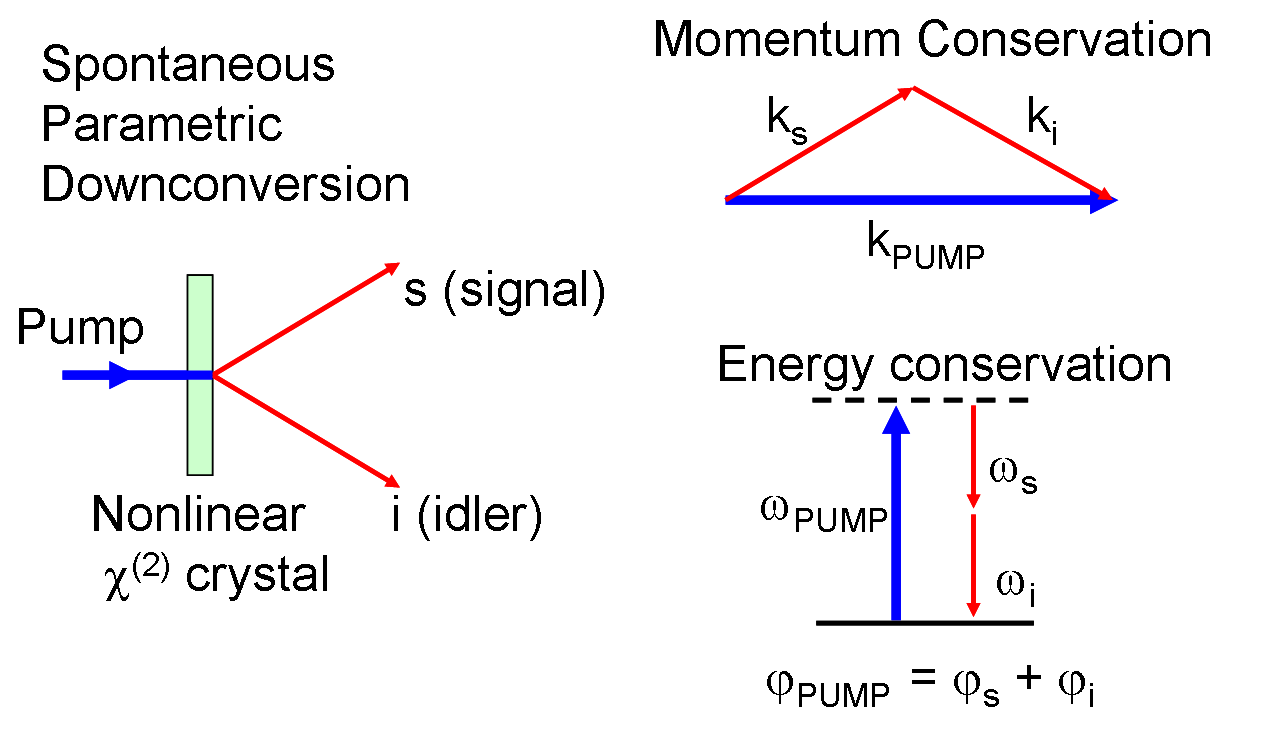
\includegraphics[width=0.7\linewidth]{images/apl2_5_spontaneous_parametric_downconversion}
	\caption{SPDC 过程示意图，守恒定律针对晶体内部的能量和动量（\cref{ref:c}）。}
	\label{fig:apl25spontaneousparametricdownconversion}
\end{figure}

由于信号光与闲置光的频率与动量为连续变量，故频率与动量纠缠虽存在，但难以利用。更常见的是通过\textbf{双折射非线性晶体}的相位匹配结构实现\textbf{偏振纠缠态}。利用晶体的双折射特性，构造出 Type-I 与 Type-II 相位匹配：

\begin{itemize}
	\item \textbf{Type-I}：pump 为 e 光，signal 和 idler 为 o 光，有
	\[
	\Delta k = k_e(\omega_p) - k_o(\omega_s) - k_o(\omega_i) = 0
	\]
	\item \textbf{Type-II}：pump 和 signal 为 o 光，idler 为 e 光，有
	\[
	\Delta k = k_o(\omega_p) - k_o(\omega_s) - k_e(\omega_i, \theta) = 0
	\]
\end{itemize}

由于 e 光与 o 光在偏振方向上不同，因此在满足相位匹配的条件下，SPDC 所产生的信号光与闲置光在偏振上表现出纠缠关系。这种由双折射非线性晶体实现的纠缠通常称为\textbf{偏振纠缠}，其在量子信息处理和基础量子力学研究中具有重要应用价值。

\subsubsection{CHSH 游戏}
\begin{enumerate}
	\item 规则
	
	有两位玩家：爱丽丝（Alice）和鲍勃（Bob）。他们事先可以协商策略（包括共享量子态），但在游戏开始后不能再通信。裁判分别给爱丽丝、鲍勃各一个比特 \( x, y \in \{0,1\} \)（可理解为随机的 00,01,10,11 四种输入各占 1/4 的概率） 。 爱丽丝、鲍勃在各自接收到输入后，须分别输出一个比特 \( a, b \in \{0,1\} \)。
	
	\textbf{胜利条件}为：
	$$ a + b = xy(mod2)   $$
	也就是说，当裁判给出 \((x,y)\)，爱丽丝和鲍勃分别输出 \((a,b)\) 后，如果满足 \(a \oplus b = x y\)，则他们在该局游戏中“赢”，否则“输”。
	
	\item 经典策略
	
	如果允许爱丽丝和鲍勃使用任何经典（含随机性但不含量子纠缠）的策略，容易证明他们最多只能以 75\%（即 3/4）概率赢下此游戏。
	
	对于确定策略：
	\begin{itemize}
		\item \textbf{Strategy: Always Send 0}
		\begin{itemize}
			\item $(x, y) = (0, 0) \Rightarrow (a, b) = (0, 0) \Rightarrow a + b = 0, \; xy = 0$
			\item $(x, y) = (0, 1) \Rightarrow (a, b) = (0, 0) \Rightarrow a + b = 0, \; xy = 0$
			\item $(x, y) = (1, 0) \Rightarrow (a, b) = (0, 0) \Rightarrow a + b = 0, \; xy = 0$
			\item $(x, y) = (1, 1) \Rightarrow (a, b) = (0, 0) \Rightarrow \textcolor{flameorange}{a + b = 0} vs. \textcolor{flameorange}{xy = 1}$
		\end{itemize}
		
		\item \textbf{Strategy: Always Send 1}
		\begin{itemize}
			\item $(x, y) = (0, 0) \Rightarrow (a, b) = (1, 1) \Rightarrow a + b = 0, \; xy = 0$
			\item $(x, y) = (0, 1) \Rightarrow (a, b) = (1, 1) \Rightarrow a + b = 0, \; xy = 0$
			\item $(x, y) = (1, 0) \Rightarrow (a, b) = (1, 1) \Rightarrow a + b = 0, \; xy = 0$
			\item $(x, y) = (1, 1) \Rightarrow (a, b) = (1, 1) \Rightarrow \textcolor{flameorange}{a + b = 0} vs. \textcolor{flameorange}{xy = 1}$
		\end{itemize}
		
		\item \textbf{Strategy: Same as Input}
		\begin{itemize}
			\item $(x, y) = (0, 0) \Rightarrow (a, b) = (0, 0) \Rightarrow a + b = 0, \; xy = 0$
			\item $(x, y) = (0, 1) \Rightarrow (a, b) = (0, 1) \Rightarrow \textcolor{flameorange}{a + b = 1} vs. \textcolor{flameorange}{xy = 0} $
			\item $(x, y) = (1, 0) \Rightarrow (a, b) = (1, 0) \Rightarrow \textcolor{flameorange}{a + b = 1} vs. \textcolor{flameorange}{xy = 0}$
			\item $(x, y) = (1, 1) \Rightarrow (a, b) = (1, 1) \Rightarrow \textcolor{flameorange}{a + b = 0} vs. \textcolor{flameorange}{xy = 1}$
		\end{itemize}
		
		\item \textbf{Strategy: Opposite of Input}
		\begin{itemize}
			\item $(x, y) = (0, 0) \Rightarrow (a, b) = (1, 1) \Rightarrow a + b = 0, \; xy = 0$
			\item $(x, y) = (0, 1) \Rightarrow (a, b) = (1, 0) \Rightarrow \textcolor{flameorange}{a + b = 1} vs. \textcolor{flameorange}{xy = 0}$
			\item $(x, y) = (1, 0) \Rightarrow (a, b) = (0, 1) \Rightarrow \textcolor{flameorange}{a + b = 1} vs. \textcolor{flameorange}{xy = 0}$
			\item $(x, y) = (1, 1) \Rightarrow (a, b) = (0, 0) \Rightarrow \textcolor{flameorange}{a + b = 0} vs. \textcolor{flameorange}{xy = 1}$
		\end{itemize}
	\end{itemize}
	
	\textbf{不确定策略是所有确定策略的凸组合}，因此由上述确定策略即可得经典策略最大胜率为75\%。
	
	\item 量子策略
	
	如果爱丽丝和鲍勃分别持有 Bell pair $\frac{\ket{00} + \ket{11}}{\sqrt{2}}$ 的一个 qubit，则通过以下策略，最大的成功概率是 85\%！
	
	先看两对正交基：
	\begin{enumerate}
		\item 
		\[
		\begin{aligned}
			\ket{\frac{\pi}{8}} &= \cos\left(\frac{\pi}{8}\right)\ket{0} + \sin\left(\frac{\pi}{8}\right)\ket{1}, \\
			\ket{\frac{5\pi}{8}} &= \cos\left(\frac{5\pi}{8}\right)\ket{0} + \sin\left(\frac{5\pi}{8}\right)\ket{1}
		\end{aligned}
		\]
		
		\item 
		\[
		\begin{aligned}
			\ket{-\frac{\pi}{8}} &= \cos\left(-\frac{\pi}{8}\right)\ket{0} + \sin\left(-\frac{\pi}{8}\right)\ket{1}, \\
			\ket{\frac{3\pi}{8}} &= \cos\left(\frac{3\pi}{8}\right)\ket{0} + \sin\left(\frac{3\pi}{8}\right)\ket{1}
		\end{aligned}
		\]
	\end{enumerate}
	
	游戏策略如下：
	\begin{itemize}
		\item $x = 0$: 爱丽丝用 $\{\ket{0}, \ket{1}\}$ 基测量，如果结果为 $\ket{0}$ 则返回 $a = 0$，如果为 $\ket{1}$ 则返回 $a = 1$
		\item $x = 1$: 爱丽丝用 $\{\ket{+}, \ket{-}\}$ 基测量，如果结果为 $\ket{+}$ 则返回 $a = 0$，如果为 $\ket{-}$ 则返回 $a = 1$
		\item $y = 0$: 鲍勃用 $\left\{ \ket{\frac{\pi}{8}}, \ket{\frac{5\pi}{8}} \right\}$ 基测量，如果结果为 $\ket{\frac{\pi}{8}}$ 则返回 $b = 0$，如果为 $\ket{\frac{5\pi}{8}}$ 则返回 $b = 1$
		\item $y = 1$: 鲍勃用 $\left\{ \ket{-\frac{\pi}{8}}, \ket{\frac{3\pi}{8}} \right\}$ 基测量，如果结果为 $\ket{-\frac{\pi}{8}}$ 则返回 $b = 0$，如果为 $\ket{\frac{3\pi}{8}}$ 则返回 $b = 1$
	\end{itemize}
	其最大成功概率为 $\cos^2\left(\frac{\pi}{8}\right) = 85\%$！
	
\end{enumerate}

\subsection{前思考题}
\begin{question}
	在实验内容 2.2 节-测试光路调节中， 为什么第 (4) 步要任意旋转半波片使符合仪计数最大？如果不旋转就去调节符合仪延时和准直器会有什么问题？
\end{question}

旋转半波片的目的是调整光子的偏振方向，使其与符合计数仪的测量基矢匹配，从而最大化符合计数。如果不旋转半波片，仅靠调整符合计数仪的延时和准直器，可能无法优化偏振态匹配，导致符合计数偏低，影响实验数据的准确性和后续分析的精度。因此，这一步是确保光路优化和实验结果可靠性的重要环节。

\begin{question}
	在实验内容 3.1 节-纠缠亮度和对比测量中， +/-基对比度可以表征实验所制备纠缠态$|\varphi \rangle = \frac{1}{\sqrt{2}}(|HH \rangle \pm e^{i \phi}|VV \rangle)$ 的哪一个参数？为什么？
\end{question}

\(+/-\)基对比度可以表征纠缠态 \(|\varphi \rangle = \frac{1}{\sqrt{2}}(|HH \rangle \pm e^{i \phi}|VV \rangle)\) 中的相位参数 \(\phi\)。这是因为在 \(+/-\)基（即 \(|+\rangle = \frac{1}{\sqrt{2}}(|H\rangle + |V\rangle)\) 和 \(|-\rangle = \frac{1}{\sqrt{2}}(|H\rangle - |V\rangle)\)）下进行测量时，符合计数的振荡行为与相位 \(\phi\) 直接相关。通过测量在 \(+/-\)基下的符合计数对比度，可以确定纠缠态的相对相位，从而判断实验制

\begin{question}
	尝试推导并解释 CHSH 游戏中量子世界如何选取最优测量基的方向？
\end{question}

在CHSH游戏中，量子世界可通过选择特定的测量基方向来最大化胜率，从而违背经典极限。

首先应当选用使用最大纠缠态，即贝尔态$|\Phi^+ \rangle = \frac{1}{\sqrt{2}}(|HH \rangle + |VV \rangle)$ 。此态在任意相同测量基下表现出完美关联。

Alice的测量基：当裁判的问题 $x=0$时，选择水平/垂直基（0°）；当$x=1$时，选择对角线基（45°）。对应的量子态投影方向为：
\[
|v_0^A \rangle = |H \rangle , \quad |v_1^A \rangle = \frac{1}{\sqrt{2}} (|H \rangle + |V \rangle)
\]

Bob的测量基：当裁判的问题$y=0$时，选择22.5°方向；当$y=1$时，选择-22.5°方向。对应的投影方向为：
\[
|v_0^B \rangle = \cos(\frac{\pi}{8}) |H \rangle + \sin(\frac{\pi}{8}) |V \rangle , \quad |v_1^B \rangle = \cos(\frac{\pi}{8}) |H \rangle - \sin(\frac{\pi}{8}) |V \rangle
\]

Alice的两个测量基夹角为45°，Bob的两个基夹角为45°，而Alice与Bob的基之间夹角为22.5°。这种对称设计使得量子关联最大化。

通过计算不同测量基组合的期望值$E(x,y)$，CHSH参数$S$可表示为：
\[
S = E(0, 22.5°) + E(0, -22.5°) + E(45°, 22.5°) - E(45°, -22.5°)
\]

可证明，当测量基满足上述角度时， $S = 2\sqrt{2} \pm $2.828，显著超过经典极限。

\begin{question}
	纠缠态制备为$|\varphi \rangle = \frac{1}{\sqrt{2}}(|HH \rangle + e^{i \phi}|VV \rangle)$ 和 $|\varphi \rangle = \frac{1}{\sqrt{2}}(|HH \rangle - e^{i \phi}|VV \rangle)$，对 CHSH 游戏的胜率以及保真度测量会产生什么影响？
\end{question}

\begin{itemize}
	\item \textbf{对胜率的影响}：
	
	如果初始态带有相位$e^{i\phi}$，即：$|\varphi_+ \rangle = \frac{1}{\sqrt{2}} (|HH \rangle + e^{i\phi} |VV \rangle)$
	
	考虑测量后纠缠态的关联函数：$\langle A_x B_y \rangle = \cos(\theta_a - \theta_B + \phi)$
	
	由于相位 $\phi$ 会改变测量结果的相关性，它影响 Bell 期望值：$S(\phi) = 2 \sqrt{2} \cos(\phi)$
	
	因此，胜率变为：$P(\phi) = \frac{1}{2} + \frac{1}{2\sqrt{2}}\cos(\phi)$
	
	\item \textbf{对保真度的影响}：
	
	保真度定义为：$F = |\langle \psi^+ | \varphi \rangle |^2$
	
	存在相位时，有：
	\[
	F_+ = |\langle \psi^+ | \varphi_+ \rangle |^2 = |\frac{1}{\sqrt{2}} (\frac{1}{\sqrt{2}}(|HH\rangle + |VV\rangle) + e^{-i\phi} \frac{1}{\sqrt{2}}(\frac{1}{\sqrt{2}}(|HH\rangle - |VV\rangle))) |^2
	\]
	\[
	\Rightarrow F_+ = \frac{1}{2} |1 + e^{-i\phi} |^2 = \frac{1 + \cos\phi}{2}
	\]
\end{itemize}

\begin{question}
	实验中会有哪些噪声会影响 CHSH 游戏的胜率？如何减小实验中的噪声？
\end{question}

在实验中，影响 CHSH 游戏胜率（即 Bell 违反程度）的噪声主要来源于 量子态制备、测量、环境干扰等因素。这些噪声会降低量子关联，使得实验结果更接近经典极限（75\%），甚至使得 Bell 不等式不再被违反。

\begin{itemize}
	\item \textbf{量子态制备误差}：
	
	CHSH 游戏通常依赖最大 Bell 纠缠态作为资源。实验中，态制备的误差可能导致量子态偏离理想 Bell 态。
	
	可能的误差来源有：由于光学路径不稳定或相干光源的相位漂移，影响测量关联；如果光学元件（波片、PBS 等）存在误差，偏振态可能偏离理想 Bell 态；单光子源效率不完美，导致实验中检测到的光子对数降低，影响统计精度。
	
	可以尝试采用主动相位锁定系统（如压电移相器或锁相环）补偿相位漂移；或者使用高质量的 PBS（偏振分束器）和波片进行偏振控制，在实验前进行系统误差校准（例如利用汤姆森散射测量偏振纯度）。
	
	\item \textbf{量子测量误差}：
	
	CHSH 游戏依赖于对量子比特的正确测量，但实验中的误差可能导致测量基的不完美。
	
	如，波片角度误差会导致投影测量方向偏离预期，使得关联性下降；光子探测器的效率不一致或探测死时间会影响测量统计；温度波动导致波片或 PBS 特性变化，进而影响测量基设置。
	
	可以尝采用高精度步进电机或压电旋转平台控制波片角度，确保测量基准确性；或采用封闭光学系统，降低环境温度变化对测量基的影响。
\end{itemize}